%% bare_conf.tex
%% V1.3
%% 2007/01/11
%% by Michael Shell
%% See:
%% http://www.michaelshell.org/
%% for current contact information.
%%
%% This is a skeleton file demonstrating the use of IEEEtran.cls
%% (requires IEEEtran.cls version 1.7 or later) with an IEEE conference paper.
%%
%% Support sites:
%% http://www.michaelshell.org/tex/ieeetran/
%% http://www.ctan.org/tex-archive/macros/latex/contrib/IEEEtran/
%% and
%% http://www.ieee.org/

%%*************************************************************************
%% Legal Notice:
%% This code is offered as-is without any warranty either expressed or
%% implied; without even the implied warranty of MERCHANTABILITY or
%% FITNESS FOR A PARTICULAR PURPOSE! 
%% User assumes all risk.
%% In no event shall IEEE or any contributor to this code be liable for
%% any damages or losses, including, but not limited to, incidental,
%% consequential, or any other damages, resulting from the use or misuse
%% of any information contained here.
%%
%% All comments are the opinions of their respective authors and are not
%% necessarily endorsed by the IEEE.
%%
%% This work is distributed under the LaTeX Project Public License (LPPL)
%% ( http://www.latex-project.org/ ) version 1.3, and may be freely used,
%% distributed and modified. A copy of the LPPL, version 1.3, is included
%% in the base LaTeX documentation of all distributions of LaTeX released
%% 2003/12/01 or later.
%% Retain all contribution notices and credits.
%% ** Modified files should be clearly indicated as such, including  **
%% ** renaming them and changing author support contact information. **
%%
%% File list of work: IEEEtran.cls, IEEEtran_HOWTO.pdf, bare_adv.tex,
%%                    bare_conf.tex, bare_jrnl.tex, bare_jrnl_compsoc.tex
%%*************************************************************************

% *** Authors should verify (and, if needed, correct) their LaTeX system  ***
% *** with the testflow diagnostic prior to trusting their LaTeX platform ***
% *** with production work. IEEE's font choices can trigger bugs that do  ***
% *** not appear when using other class files.                            ***
% The testflow support page is at:
% http://www.michaelshell.org/tex/testflow/



% Note that the a4paper option is mainly intended so that authors in
% countries using A4 can easily print to A4 and see how their papers will
% look in print - the typesetting of the document will not typically be
% affected with changes in paper size (but the bottom and side margins will).
% Use the testflow package mentioned above to verify correct handling of
% both paper sizes by the user's LaTeX system.
%
% Also note that the "draftcls" or "draftclsnofoot", not "draft", option
% should be used if it is desired that the figures are to be displayed in
% draft mode.
%
\documentclass[10pt,conference,compsocconf]{IEEEtran}
%\documentclass[10pt]{IEEEtran}
\usepackage{times}
\usepackage{color}
\usepackage{caption}
\usepackage{graphicx}
\usepackage{hyperref}
\usepackage{etoolbox}
\usepackage[dvipsnames]{xcolor}
\usepackage{authblk}
\usepackage{blindtext}


\captionsetup{font=footnotesize,justification=centering,labelsep=period}

% Add the compsoc option for Computer Society conferences.
%
% If IEEEtran.cls has not been installed into the LaTeX system files,
% manually specify the path to it like:
% \documentclass[conference]{../sty/IEEEtran}





% Some very useful LaTeX packages include:
% (uncomment the ones you want to load)


% *** MISC UTILITY PACKAGES ***
%
%\usepackage{ifpdf}
% Heiko Oberdiek's ifpdf.sty is very useful if you need conditional
% compilation based on whether the output is pdf or dvi.
% usage:
% \ifpdf
%   % pdf code
% \else
%   % dvi code
% \fi
% The latest version of ifpdf.sty can be obtained from:
% http://www.ctan.org/tex-archive/macros/latex/contrib/oberdiek/
% Also, note that IEEEtran.cls V1.7 and later provides a builtin
% \ifCLASSINFOpdf conditional that works the same way.
% When switching from latex to pdflatex and vice-versa, the compiler may
% have to be run twice to clear warning/error messages.






% *** CITATION PACKAGES ***
%
%\usepackage{cite}
% cite.sty was written by Donald Arseneau
% V1.6 and later of IEEEtran pre-defines the format of the cite.sty package
% \cite{} output to follow that of IEEE. Loading the cite package will
% result in citation numbers being automatically sorted and properly
% "compressed/ranged". e.g., [1], [9], [2], [7], [5], [6] without using
% cite.sty will become [1], [2], [5]--[7], [9] using cite.sty. cite.sty's
% \cite will automatically add leading space, if needed. Use cite.sty's
% noadjust option (cite.sty V3.8 and later) if you want to turn this off.
% cite.sty is already installed on most LaTeX systems. Be sure and use
% version 4.0 (2003-05-27) and later if using hyperref.sty. cite.sty does
% not currently provide for hyperlinked citations.
% The latest version can be obtained at:
% http://www.ctan.org/tex-archive/macros/latex/contrib/cite/
% The documentation is contained in the cite.sty file itself.






% *** GRAPHICS RELATED PACKAGES ***
%
\ifCLASSINFOpdf
  % \usepackage[pdftex]{graphicx}
  % declare the path(s) where your graphic files are
  % \graphicspath{{../pdf/}{../jpeg/}}
  % and their extensions so you won't have to specify these with
  % every instance of \includegraphics
  % \DeclareGraphicsExtensions{.pdf,.jpeg,.png}
\else
  % or other class option (dvipsone, dvipdf, if not using dvips). graphicx
  % will default to the driver specified in the system graphics.cfg if no
  % driver is specified.
  % \usepackage[dvips]{graphicx}
  % declare the path(s) where your graphic files are
  % \graphicspath{{../eps/}}
  % and their extensions so you won't have to specify these with
  % every instance of \includegraphics
  % \DeclareGraphicsExtensions{.eps}
\fi
% graphicx was written by David Carlisle and Sebastian Rahtz. It is
% required if you want graphics, photos, etc. graphicx.sty is already
% installed on most LaTeX systems. The latest version and documentation can
% be obtained at: 
% http://www.ctan.org/tex-archive/macros/latex/required/graphics/
% Another good source of documentation is "Using Imported Graphics in
% LaTeX2e" by Keith Reckdahl which can be found as epslatex.ps or
% epslatex.pdf at: http://www.ctan.org/tex-archive/info/
%
% latex, and pdflatex in dvi mode, support graphics in encapsulated
% postscript (.eps) format. pdflatex in pdf mode supports graphics
% in .pdf, .jpeg, .png and .mps (metapost) formats. Users should ensure
% that all non-photo figures use a vector format (.eps, .pdf, .mps) and
% not a bitmapped formats (.jpeg, .png). IEEE frowns on bitmapped formats
% which can result in "jaggedy"/blurry rendering of lines and letters as
% well as large increases in file sizes.
%
% You can find documentation about the pdfTeX application at:
% http://www.tug.org/applications/pdftex





% *** MATH PACKAGES ***
%
%\usepackage[cmex10]{amsmath}
% A popular package from the American Mathematical Society that provides
% many useful and powerful commands for dealing with mathematics. If using
% it, be sure to load this package with the cmex10 option to ensure that
% only type 1 fonts will utilized at all point sizes. Without this option,
% it is possible that some math symbols, particularly those within
% footnotes, will be rendered in bitmap form which will result in a
% document that can not be IEEE Xplore compliant!
%
% Also, note that the amsmath package sets \interdisplaylinepenalty to 10000
% thus preventing page breaks from occurring within multiline equations. Use:
%\interdisplaylinepenalty=2500
% after loading amsmath to restore such page breaks as IEEEtran.cls normally
% does. amsmath.sty is already installed on most LaTeX systems. The latest
% version and documentation can be obtained at:
% http://www.ctan.org/tex-archive/macros/latex/required/amslatex/math/





% *** SPECIALIZED LIST PACKAGES ***
%
%\usepackage{algorithmic}
% algorithmic.sty was written by Peter Williams and Rogerio Brito.
% This package provides an algorithmic environment fo describing algorithms.
% You can use the algorithmic environment in-text or within a figure
% environment to provide for a floating algorithm. Do NOT use the algorithm
% floating environment provided by algorithm.sty (by the same authors) or
% algorithm2e.sty (by Christophe Fiorio) as IEEE does not use dedicated
% algorithm float types and packages that provide these will not provide
% correct IEEE style captions. The latest version and documentation of
% algorithmic.sty can be obtained at:
% http://www.ctan.org/tex-archive/macros/latex/contrib/algorithms/
% There is also a support site at:
% http://algorithms.berlios.de/index.html
% Also of interest may be the (relatively newer and more customizable)
% algorithmicx.sty package by Szasz Janos:
% http://www.ctan.org/tex-archive/macros/latex/contrib/algorithmicx/




% *** ALIGNMENT PACKAGES ***
%
%\usepackage{array}
% Frank Mittelbach's and David Carlisle's array.sty patches and improves
% the standard LaTeX2e array and tabular environments to provide better
% appearance and additional user controls. As the default LaTeX2e table
% generation code is lacking to the point of almost being broken with
% respect to the quality of the end results, all users are strongly
% advised to use an enhanced (at the very least that provided by array.sty)
% set of table tools. array.sty is already installed on most systems. The
% latest version and documentation can be obtained at:
% http://www.ctan.org/tex-archive/macros/latex/required/tools/


%\usepackage{mdwmath}
%\usepackage{mdwtab}
% Also highly recommended is Mark Wooding's extremely powerful MDW tools,
% especially mdwmath.sty and mdwtab.sty which are used to format equations
% and tables, respectively. The MDWtools set is already installed on most
% LaTeX systems. The lastest version and documentation is available at:
% http://www.ctan.org/tex-archive/macros/latex/contrib/mdwtools/


% IEEEtran contains the IEEEeqnarray family of commands that can be used to
% generate multiline equations as well as matrices, tables, etc., of high
% quality.


%\usepackage{eqparbox}
% Also of notable interest is Scott Pakin's eqparbox package for creating
% (automatically sized) equal width boxes - aka "natural width parboxes".
% Available at:
% http://www.ctan.org/tex-archive/macros/latex/contrib/eqparbox/





% *** SUBFIGURE PACKAGES ***
%\usepackage[tight,footnotesize]{subfigure}
% subfigure.sty was written by Steven Douglas Cochran. This package makes it
% easy to put subfigures in your figures. e.g., "Figure 1a and 1b". For IEEE
% work, it is a good idea to load it with the tight package option to reduce
% the amount of white space around the subfigures. subfigure.sty is already
% installed on most LaTeX systems. The latest version and documentation can
% be obtained at:
% http://www.ctan.org/tex-archive/obsolete/macros/latex/contrib/subfigure/
% subfigure.sty has been superceeded by subfig.sty.



%\usepackage[caption=false]{caption}
%\usepackage[font=footnotesize]{subfig}
% subfig.sty, also written by Steven Douglas Cochran, is the modern
% replacement for subfigure.sty. However, subfig.sty requires and
% automatically loads Axel Sommerfeldt's caption.sty which will override
% IEEEtran.cls handling of captions and this will result in nonIEEE style
% figure/table captions. To prevent this problem, be sure and preload
% caption.sty with its "caption=false" package option. This is will preserve
% IEEEtran.cls handing of captions. Version 1.3 (2005/06/28) and later 
% (recommended due to many improvements over 1.2) of subfig.sty supports
% the caption=false option directly:
%\usepackage[caption=false,font=footnotesize]{subfig}
%
% The latest version and documentation can be obtained at:
% http://www.ctan.org/tex-archive/macros/latex/contrib/subfig/
% The latest version and documentation of caption.sty can be obtained at:
% http://www.ctan.org/tex-archive/macros/latex/contrib/caption/




% *** FLOAT PACKAGES ***
%
%\usepackage{fixltx2e}
% fixltx2e, the successor to the earlier fix2col.sty, was written by
% Frank Mittelbach and David Carlisle. This package corrects a few problems
% in the LaTeX2e kernel, the most notable of which is that in current
% LaTeX2e releases, the ordering of single and double column floats is not
% guaranteed to be preserved. Thus, an unpatched LaTeX2e can allow a
% single column figure to be placed prior to an earlier double column
% figure. The latest version and documentation can be found at:
% http://www.ctan.org/tex-archive/macros/latex/base/



%\usepackage{stfloats}
% stfloats.sty was written by Sigitas Tolusis. This package gives LaTeX2e
% the ability to do double column floats at the bottom of the page as well
% as the top. (e.g., "\begin{figure*}[!b]" is not normally possible in
% LaTeX2e). It also provides a command:
%\fnbelowfloat
% to enable the placement of footnotes below bottom floats (the standard
% LaTeX2e kernel puts them above bottom floats). This is an invasive package
% which rewrites many portions of the LaTeX2e float routines. It may not work
% with other packages that modify the LaTeX2e float routines. The latest
% version and documentation can be obtained at:
% http://www.ctan.org/tex-archive/macros/latex/contrib/sttools/
% Documentation is contained in the stfloats.sty comments as well as in the
% presfull.pdf file. Do not use the stfloats baselinefloat ability as IEEE
% does not allow \baselineskip to stretch. Authors submitting work to the
% IEEE should note that IEEE rarely uses double column equations and
% that authors should try to avoid such use. Do not be tempted to use the
% cuted.sty or midfloat.sty packages (also by Sigitas Tolusis) as IEEE does
% not format its papers in such ways.





% *** PDF, URL AND HYPERLINK PACKAGES ***
%
%\usepackage{url}
% url.sty was written by Donald Arseneau. It provides better support for
% handling and breaking URLs. url.sty is already installed on most LaTeX
% systems. The latest version can be obtained at:
% http://www.ctan.org/tex-archive/macros/latex/contrib/misc/
% Read the url.sty source comments for usage information. Basically,
% \url{my_url_here}.





% *** Do not adjust lengths that control margins, column widths, etc. ***
% *** Do not use packages that alter fonts (such as pslatex).         ***
% There should be no need to do such things with IEEEtran.cls V1.6 and later.
% (Unless specifically asked to do so by the journal or conference you plan
% to submit to, of course. )


% correct bad hyphenation here
\hyphenation{op-tical net-works semi-conduc-tor}

%\parskip 6pt plus 2pt minus 1pt
\parskip 3pt plus 2pt minus 1pt

\pagestyle{empty}

\begin{document}
\pagenumbering{gobble}
%
% paper title
% can use linebreaks \\ within to get better formatting as desired
\title{\textbf{\Large Computer Vision-based System for Impaired Human Vision Compensation}} % \\[-1.5ex] and subtitle}\\[0.2ex]}

% author names and affiliations
% use a multiple column layout for up to three different
% affiliations
%\author{\IEEEauthorblockN{~\\[-0.4ex]\large Povilas Daniu\v{s}is\\[0.3ex]\normalsize}
%\IEEEauthorblockA{Vilnius Gediminas Technical University\\
%Vilnius, Lithuania}
%\and
%\IEEEauthorblockN{~\\[-0.4ex]\large Audrius Indriulionis\\[0.3ex]\normalsize}
%\IEEEauthorblockA{Vilnius Gediminas Technical University,\\
%Nature Research Center, Vilnius, Lithuania}
%\and
%\IEEEauthorblockN{~\\[-0.4ex]\large Andrius Budrionis\\[0.3ex]\normalsize}
%\IEEEauthorblockA{Vilnius Gediminas Technical University\\
%Vilnius, Lithuania\\
%Norwegian Centre for E-health Research\\
%University Hospital of North Norway\\
%Tromsø, Norway}
%\and
%\author{\IEEEauthorblockN{~\\[-0.4ex]\large Darius Plikynas\\[0.3ex]%\normalsize}
%\IEEEauthorblockA{Vilnius Gediminas Technical University\\
%Vilnius, Lithuania}
%}}

% conference papers do not typically use \thanks and this command
% is locked out in conference mode. If really needed, such as for
% the acknowledgment of grants, issue a \IEEEoverridecommandlockouts
% after \documentclass

% for over three affiliations, or if they all won't fit within the width
% of the page, use this alternative format:
% 
%\author{\IEEEauthorblockN{Povilas Daniu\v{s}is\IEEEauthorrefmark{1},
%Andrius Budrionis\IEEEauthorrefmark{1}\IEEEauthorrefmark{2},
%Audrius Indriulionis\IEEEauthorrefmark{1}\IEEEauthorrefmark{3} and 
%Darius Plikynas\IEEEauthorrefmark{1}}
%\IEEEauthorblockA{\IEEEauthorrefmark{1}Vilnius Gediminas Technical University,\\
%Vilnius, Lithuania.
%}
%\IEEEauthorblockA{\IEEEauthorrefmark{2}Norwegian Centre for E-health Research, University Hospital of North Norway,\\
%Troms\o, Norway.}
%\IEEEauthorblockA{\IEEEauthorrefmark{3}Nature Research Center,\\ 
%Vilnius, Lithuania.
%}}

% first version of affilation
%\author{\IEEEauthorblockN{Povilas Daniu\v{s}is\IEEEauthorrefmark{1},
%Andrius Budrionis\IEEEauthorrefmark{1}\IEEEauthorrefmark{2},
%Audrius Indriulionis\IEEEauthorrefmark{1}\IEEEauthorrefmark{3} and 
%Darius Plikynas\IEEEauthorrefmark{1}}
%\IEEEauthorblockA{\IEEEauthorrefmark{1} Department of Business Technologies  and Entrepreneurship\\ Vilnius Gediminas Technical University\\
%Vilnius, Lithuania}
%\IEEEauthorblockA{\IEEEauthorrefmark{2}Norwegian Centre for E-health Research\\ University %Hospital of North Norway\\
%Troms\o, Norway}
%\IEEEauthorblockA{\IEEEauthorrefmark{3} Laboratory of Quaternary Research\\ Nature Research Centre %\\ Vilnius, Lithuania\\
%Email: \IEEEauthorrefmark{1} {povilas.daniusis, andrius.budrionis, audrius.indriulionis, %darius.plikynas} @vgtu.lt}}

%%%%\IEEEauthorrefmark{2}andrius.budrionis@vgtu.lt,
%%%%\IEEEauthorrefmark{3}audrius.indriulionis@vgtu.lt,
%%%\\\IEEEauthorrefmark{4}darius.plikynas@vgtu.lt}}
% second version of affilation
\author[1]{Povilas Daniu\v{s}is}
\author[1,2]{Andrius Budrionis}
\author[1,3]{ Audrius Indriulionis}
\author[1]{ Darius Plikynas}
\affil[1]{Department of Business Technologies  and Entrepreneurship 
\authorcr Gediminas Technical University 
\authorcr Vilnius, Lithuania
\authorcr Email: {\tt \{povilas.daniusis, darius.plikynas\}@vgtu.lt}\vspace{1.5ex}}
\affil[2]{Norwegian Centre for E-health Research 
\authorcr University Hospital of North Norway
\authorcr Troms\o, Norway
 \authorcr Email: {\tt andrius.budrionis@ehealthresearch.no} \vspace{1.5ex}} 
\affil[3]{Laboratory of Quaternary Research 
\authorcr  Nature Research Centre
\authorcr Vilnius, Lithuania
\authorcr Email: {\tt audrius.indriulionis@gmail.com}}


% use for special paper notices
%\IEEEspecialpapernotice{(Invited Paper)}




% make the title area
\maketitle

\setlength{\parskip}{0.1em} % reduce spacings between paragraphs




\begin{abstract}
%\boldmath
This paper presents a high-level architecture of a computer vision-based system for partial compensation of lost or impaired human vision. It combines standard smartphone device, external deep learning-based image processing infrastructure and audio/tactile user interface. The proposed architecture is based on input from user-centered design process, involving end-users into system development. The paper discusses user needs and expectations for electronic travelling aids for the blind and highlights limitations of the existing solutions. The suggested architecture may be used as a basis for developing computer vision-based tools for visually impaired individuals.   
\end{abstract}
% IEEEtran.cls defaults to using nonbold math in the Abstract.
% This preserves the distinction between vectors and scalars. However,
% if the conference you are submitting to favors bold math in the abstract,
% then you can use LaTeX's standard command \boldmath at the very start
% of the abstract to achieve this. Many IEEE journals/conferences frown on
% math in the abstract anyway.

% no keywords

\begin{IEEEkeywords}
computer vision; deep learning; mobile application; aid for blind and visually impaired; audio feedback; tactile feedback; impaired human vision compensation; user-centered design.%
\end{IEEEkeywords}
% For peer review papers, you can put extra information on the cover
% page as needed:
% \ifCLASSOPTIONpeerreview
% \begin{center} \bfseries EDICS Category: 3-BBND \end{center}
% \fi
%
% For peerreview papers, this IEEEtran command inserts a page break and
% creates the second title. It will be ignored for other modes.
\IEEEpeerreviewmaketitle
\section{Introduction}
\label{sec:introduction}
More than $250$ million people worldwide have moderate to severe vision impairment, while ($\approx 36$ million are blind) \cite{Bourne}. During the past decades significant effort was devoted to develop computer vision and other sensor-based aids (e.g., \cite{Caraiman}-\cite{Zientara}) for helping the blind and visually impaired users to perceive the surrounding world better. However, computer vision is a rapidly evolving field; systems based on the aforementioned approaches become outdated in a relatively short time and often lack accuracy and reliability in real-world conditions in comparison to the state-of-the-art technologies. In this article, we describe a system, which employs modern computer vision techniques for compensation of lost or impaired vision function in humans. Many of the previously proposed electronic aids for the blind count on highly specialized hardware, for instance smart glasses \cite{Zientara}, Microsoft Kinnect sensors \cite{Owayjan}, helmet-mounted photo sensors and cameras \cite{Dunai}. Such systems often lack convenience and bring additional complexity into daily tasks, which visually impaired people currently manage by the help of a white cane. This project puts major emphasis on developing a tool, which seamlessly integrates with the hardware visually impaired persons already have on-hand and are used to (smartphone). This paper describes a high level architecture of the technology aid for visually impaired people utilizing the latest achievements in the field of computer vision. 

\textcolor{red}{We begin our presentation with Section~\ref{sec:method}, describing the methodological foundations of this research. Section~\ref{sec:results} focuses on the architecture of the suggested human vision compensation system. Finally, Section~\ref{sec:discussion} summarizes and discusses the results of the conducted analysis.}


\section{Method}
\label{sec:method}

Following the principles of the participatory design \cite{Kensing}\cite{Carroll} we included end-users into system design process. Two visually impaired persons participated in discussion and focus group meetings together with the project team to identify the key properties of the solution. During the six discussion sessions, major attention was paid to:
\begin{enumerate}
\item Functionality and key features of the solution addressing real-life scenarios of visually impaired persons;
\item Technical feasibility, connecting user needs to the latest development in computer vision and assistive technologies;
\item Interface between the visually impaired person and the assistive technology;
\item Appearance, usability and potential costs of the proposed product. 
\end{enumerate}
Participatory design process included testing of assistive technologies for the blind and visually impaired people using widely available mobile phone apps like Seeing AI, BlindWays, Be My Eyes, Aipoly Vision, TapTapSee, etc.
%Design process included testing of the existing mobile phone apps (Seeing AI, BlindWays, Be My Eyes, Aipoly Vision, TapTapSee) for assisting visually impaired people. 
Semi-structured tests were performed by visually impaired participants and researchers from the project group. Strengths and weaknesses of the existing solutions are reflected in the design of the proposed system. 

%Andrius: If we leave this section in manuscript, we should probably have a section addressing the findings of the reviews in the Results section.
%Darius
To have an overview on research progress on assistive technologies for the blind during the last ten years, a systematic literature review in three major research databases (Medline, IEEE xplore and ACM DL) was conducted. It revealed increasing research interest in the field (84 related publications were identified, while 17 were characterized as highly relevant for this project) and provided better understanding of the state-of-the-art in applying computer vision technologies to address the needs of the blind. 
%In order to better understand the applicability of modern computer vision technologies, we also conducted comprehensive analysis of recent advantages in the topic.
%we carried out  systemic review of research articles in databases like  Medline, IEEE xplore, ACM DL.  
The review was extended to relevant patents and patent applications worldwide. The search was performed in the following databases: EspaceNet, GooglePatents, USPTO, PatentScope, FreePatentsOnline. It revealed several technological trends in the field of assistive technologies for the blind persons.
%Systemic review of the relevant patents and patent applications worldwide was performed using online services of the following databases: EspaceNet, GooglePatents, USPTO, PatentScope, FreePatentsOnline. It revealed several main technological trends in the area of assistive technologies for the blind persons. 
Based on the aforementioned reviews, our insights are presented in the Results section.




\section{Results}
\label{sec:results}

User-centered design sessions with visually impaired persons and analysis of the aforementioned data sources provided substantial input for the design of the proposed system (Figure~\ref{fig:schematics}). The process made it clear that understanding of the user needs was limited in the project team. Based on the results of the user-centered design process, scientific publications and patent analysis, we present the outline of the system for impaired human vision compensation. 

The key part of the proposed system is a smartphone device, connecting User interface (UI) and data processing components into a well-functioning ecosystem. Smartphone was selected due to its high availability and capability to perform required computations or forward visual information for processing to the external server via the Internet.

% Man atrodo, kad cia du esminiai sistemos komponentai, kuriuos reiktu akcentuoti:
%The cornerstones of the proposed solution are its user interface and vision processing system, consisting of external server, equipped with a set of computer vision algorithms, selected and combined according to the above methodology.

% User interface
UI consists of a wearable forehead belt, integrating RGB and depth cameras, Inertial measurement unit (IMU), tactile feedback device and bone conduction headphones. Although more expensive than standard ones, bone conduction headphones do not block the ears and allow the user to perceive audio information from the surrounding environment and the system at the same time, which is essential for the visually impaired people. 


However, some types of guidance information may be more efficiently perceived through tactile feedback device than audio channel. For instance, indicating the direction of a detected object with a vibromotor on the corresponding area on the forehead belt, instead of providing audio description. More research is needed to clarify how various types of guidance information should be represented to the user in the most convenient and efficient way. \textcolor{red}{ For instance, the detected objects could be presented to the user in a configurable order, based on the subjective importance of particular object classes or other personalized criteria.} USB and Wifi data links can be used for bidirectional data transmission between UI and smartphone component.


% External vision processor
%visus sutrumpinimus reikia pirma parasyt pilnai, pvz Neural Network (NN)
Although modern high-end smartphones are powerful computational devices, many computer vision algorithms  require hardware of significantly higher processing capabilities (e.g., a server equipped with a high-end Graphics Processing Unit (GPU)). Therefore, an external server is used for live video data processing. In our design we envision a computational server hosting a set of computer vision algorithms implemented and exposed via web services: faster Regions with Convolutional Neural Network features (faster R-CNN) object detector \cite{Ren}, trained to detect important objects, Convolutional Neural Network (CNN) and Recurrent Neural Network-based (RNN) scene descriptor \cite{Liu}, which provides textual annotation of a given RGB image, place recognition \cite{Ohn-Bar}, face detection and recognition \cite{Amos}, obstacle detection \cite{Laina}, action recognition \cite{Valor}, among others. After video analysis is completed on the server side, results are transmitted back to the smartphone component and represented to the user through the aforementioned UI.

% How user controls system
The user interacts with the system through gestures, voice commands or specifically designed user interface on the smartphone. User input is required for selecting operation mode of the system, i.e., switching between Optical Character Recognition (OCR), currency recognition, object detection, navigation aid and other available functions. 

% Potential applications
Social networking functionality was highlighted as a potentially important feature allowing other users/volunteers contribute to up-to-date and high quality guidance (for instance, temporary road works) with exact location and description. Navigating around such obstacles can be challenging for computer vision-based tools and may decrease user's trust in the tool. Integration of additional information from other users, governmental organizations and volunteers could be of high value for the visually impaired people.

%\begin{wrapfigure}{r}{0.4\textwidth}
\begin{figure}
  \begin{center}
    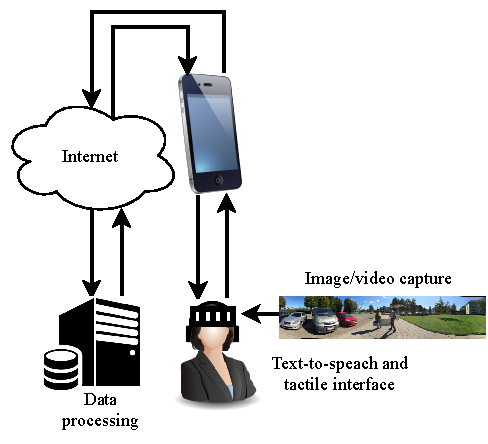
\includegraphics[scale=1.0]{./img/cropped_diagram.pdf}  
  \end{center}
  \caption{Schematics of vision compensation device.}
  \label{fig:schematics}
\end{figure}



Discussions on the key features of the proposed solution revealed a gap between the functionality of the existing tools, which are often focused on advanced navigation and scene description features, and actual user needs. For example, the end-users highlighted that a simplistic solution for navigating is lacking. Major focus was put on an easy-to-use and minimalistic tool, which can be trusted. Reliable object detection, direction and approximate distance to an obstacle were highlighted as the main requirements. To our surprise, only 5-8 distinctive object classes (for instance, buss stop, pedestrian crossing, doors, stairs, etc.) were of major importance while navigating. Additional information, such as type of a passing car, blossoming flowers in the park or a person riding a bicycle was considered as overwhelming and distractive. 

%Povilai, paziurek ar cia viskas OK, pridek ka nors nuo saves
% Pamineti mobilenet ir pan.
Computer vision technology is under rapid development and during the last years made a major breakthrough in performance and efficiency. Deep learning neural networks, which are de facto standard in modern image/video processing in many real-world problems allow to achieve accuracies, similar to that of human decision (e.g., face recognition \cite{Amos}, object detection \cite{Ren}, among others). These models are now well supported by software libraries (e.g., \cite{Tensorflow}) and dedicated processing hardware is built-in even in relatively low-power computational devices, such as smartphones. These devices are also equipped with 4G Internet connectivity and sufficient computational power to perform partial or in certain cases even full visual data processing locally. The maturity of the aforementioned technologies suggest that our proposed computational aid for visually impaired persons may be highly feasible. 


The cornerstone of this project is the interface between the visually impaired person and the assistive technology. We are proposing a combination of audio and tactile feedback, which may improve the interaction between the assistive technology and the user. Similar interfaces were suggested by research communities earlier \cite{Poggi}\cite{Zientara}, however, existing knowledge on user preferences and evaluation of various options of tactile feedback (types of actuators, placement on the body, frequencies, strength, etc.) is limited. 

Appearance, usability and cost of the end product are of major importance to the users. The proposed assistive technology should supplement the tool that visually impaired persons used for decades - the white cane. Using a white cane requires little to no training, has very low costs and is relatively reliable. It provides information on the surrounding objects 1-2 meters in front of the user. While the cane can be used to detect nearby obstacles, electronic travel aid could be beneficial for longer range (2-10m) route planning and object detection. However, it should integrate seamlessly into the existing navigation practices of visually impaired people. 


 
\section{Discussion}
\label{sec:discussion}


This paper outlined a high-level architecture of a computer vision-based system, which may help to partially compensate impaired or lost human vision. The main advantages of therein suggested system are: ability to use efficient (but still computationally intensive) modern computer vision algorithms via the Internet connection and present the output of the video processing to the user through a combined audio/tactile interface. 

Similar functionality has been previously addressed by research communities \cite{Caraiman}-\cite{Zientara} and industry \cite{orcam}\cite{horus}. The main difference between the aforementioned commercial solutions and the proposed system is the ability to utilize external resources for computationally intensive image and video processing tasks. While the availability of the computational power could be seen as the main advantage, it comes with high cost - dependency on a well-functioning mobile broadband. The development of the high-speed mobile networks (4G and 5G in the nearest future) is likely to make the major limitation of the proposed architecture obsolete, especially in densely populated areas containing many hazards for the blind. On the other side, increasing computational power of smartphones may also allow to perform more advanced image and video processing locally. \textcolor{red}{Although not always technically feasible, local  processing is especially important in low connectivity areas to ensure at least partial functionality of the system.} Combined audio/tactile interface may also be more convenient for the users, allowing to provide feedback in a more efficient way than using tactile or audio interfaces separately. 

Both open source (e.g., \cite{Tensorflow}) and state of the art commercial computer vision software libraries (e.g., \cite{Verilook}) may be applied implementing the suggested architecture. Moreover, a detailed specification of the suggested hardware components, following open hardware approach (providing an open repository containing a detailed list of electronic components, schematics, and 3D models of mechanical parts) could provide a solid basis for semi-standard reference platform for the researchers in the field.


It is important to emphasize that the suggested system does not aim to replace the main travelling aid of visually impaired people - the white cane. Instead, this computer vision tool aims to enhance and push the perception of the surrounding environment boundary from 1-2 meters (achieved by using the white cane) to 2-10 meters. It may improve route planning and identification of objects of interest (for instance, doors, stairs, elevators, bus stops, etc.). This functionality corresponds with the main requirement for electronic travelling aids highlighted by the end-users - direction and distance estimation to a selected object. The proposed hardware architecture can be used as basis for various computer vision-based software modules, aiming to assist visually impaired users in daily activities (e.g., outdoor/indoor navigation, object/face recognition, obstacle detection, etc.). 


The proposed architecture is based on several assumptions, which may be characterized as limitations of the system. For instance, technical feasibility of the solution is dependent on the availability of high bandwidth Internet connection ensuring access to high-power data processing components. Insufficient bandwidth may result in latency, which may not be tolerated by the users.  

Economical feasibility of the proposed solution may also be questioned. Advanced technology (high-end smartphone, depth camera, tactile feedback device, bone conduction headphones) is needed to ensure reliable functioning of the system. A combination of such components may be perceived as costly by the end users. More research is needed to demonstrate the cost-benefit analysis of the system in real-world scenarios. 

\section*{Acknowledgment}
This research is/was funded by the European Regional Development Fund according to the supported activity ‘Research Projects Implemented by World-class Researcher Groups’ under Measure No. 01.2.2-LMT-K-718.
%The authors would like to thank...





% trigger a \newpage just before the given reference
% number - used to balance the columns on the last page
% adjust value as needed - may need to be readjusted if
% the document is modified later
%\IEEEtriggeratref{8}
% The "triggered" command can be changed if desired:
%\IEEEtriggercmd{\enlargethispage{-5in}}

% references section

% can use a bibliography generated by BibTeX as a .bbl file
% BibTeX documentation can be easily obtained at:
% http://www.ctan.org/tex-archive/biblio/bibtex/contrib/doc/
% The IEEEtran BibTeX style support page is at:
% http://www.michaelshell.org/tex/ieeetran/bibtex/
%\bibliographystyle{IEEEtran}
% argument is your BibTeX string definitions and bibliography database(s)
%\bibliography{IEEEabrv,../bib/paper}
%
% <OR> manually copy in the resultant .bbl file
% set second argument of \begin to the number of references
% (used to reserve space for the reference number labels box)
%
% As suggested below, edit bibtemplate_samples.bib to reflect
% your bibliography. See bibtemplate.text for referencing.
%

\bibliographystyle{IEEEtran}
%\bibliography{bibtemplate_samples}


\begin{thebibliography}{99}

\bibitem{Bourne} R. R. A. Bourne et al. Vision Loss Expert Group. Magnitude, temporal trends, and projections of the global prevalence of blindness and distance and near vision impairment: a systematic review and meta-analysis. Lancet Glob Health. Vol. 5(9), pp. 888-897, 2017.


\bibitem{Caraiman} S. Caraiman et al. A. Computer Vision for the Visually Impaired: the Sound of Vision System. IEEE International Conference on Computer Vision Workshops, pp. 1480-1489, 2017.

\bibitem{Csapo} A. Csap\'{o}, G. Wers\'{e}nyi, H. Nagy, and T. A. Stockman. A survey of assistive technologies and applications for blind users on mobile platforms: a review and foundation for research. Journal on Multimodal User Interfaces. Vol. 9, issue 4,  pp. 275-286, 2015.


\bibitem{Poggi} M. Poggi and S. Mattoccia. A wearable mobility aid for the visually impaired based on embedded 3d vision and deep learning. Proceeding of IEEE Symposium on Compututers and Communication, pp. 208-213, 2016.

\bibitem{Zientara} P. A. Zientara at al. Third Eye: A shopping assistant for the visually impaired. Computer Vol. 50, Issue 2, pp. 16-24, 2017.


\bibitem{Owayjan} M. Owayjan, A. Hayek, H. Nassrallah, and M. Eldor. Smart Assistive Navigation System for Blind and Visually Impaired Individuals. 2015 International Conference on Advances in Biomedical Engineering (ICABME), pp. 162-165, 2015.


\bibitem{Dunai} L. D. Dunai, I. L. Lengua, I. Tortajada, and F. B. Simon. Obstacle detectors for visually impaired people. 2014 International Conference on Optimization of Electrical and Electronic Equipment (OPTIM),  pp. 809-816, 2014.

\bibitem{Kensing} F. Kensing, J. Simonsen, and K. B\o dker. MUST: A Method for Participatory Design. Human Computer Interaction, vol. 13, no. 2, pp. 167-198, Jun. 1998.


\bibitem{Carroll} J. M. Carroll and M. B. Rosson. Participatory design in community informatics. Des. Stud., vol. 28, no. 3, pp. 243-261, May 2007.

\bibitem{Ren} Sh. Ren, K. He, R. Girshick, and J. Sun.  Faster R-CNN: Towards real-time object detection with region proposal networks. In Advances in neural information processing systems, pp. 91-99, 2015.




\bibitem{Liu} Ch. Liu, J. Mao, F. Sha, and A. Yuille. Attention Correctness in Neural Image Captioning. Proceedings of the Thirty-First AAAI Conference on Artificial Intelligence, pp. 4176-4182, 2017.

\bibitem{Ohn-Bar} E. Ohn-Bar, K. Kitani, and Ch. Asakawa. Personalized Dynamics Models for Adaptive Assistive Navigation Interfaces. arXiv:1804.04118, [cs.LG], 2018.




\bibitem{Amos} B. Amos, B. Ludwiczuk, and M. Satyanarayanan. Openface: A general-purpose face recognition library with mobile applications. Technical report, CMU-CS-16-118, CMU School of Computer Science, 2016.


\bibitem{Laina} I. Laina, C. Rupprecht, V. Belagiannis, F. Tombari, and N. Navab. Deeper depth prediction with fully convolutional residual networks. Fourth International Conference on 3D Vision (3DV), pp. 239-248, 2016.

%-------------------

\bibitem{Valor} G. Varol, I. Laptev, and C. Schmid. Long-Term Temporal Convolutions for Action Recognition.  IEEE Transactions on Pattern Analysis and Machine Intelligence. Vol. 40, issue 6, pp. 1510-1517, 2016.

\bibitem{Tensorflow} M. Abadi et al. TensorFlow: Large-Scale Machine Learning on Heterogeneous Distributed Systems, arXiv:1603.04467, 2016. 

%-------------------

\bibitem{orcam} Orcam. MyEye 2.0. [Online]. Available from https://www.orcam.com [retrieved: 1 2019].

\bibitem{horus} Horus. Horus system. [Online]. Available from http://www.horus.tech [retrieved: 1 2019].

\bibitem{Verilook} Neurotechnology, VeriLook SDK. [Online]. Available from https://www.neurotechnology.com/verilook.html [retrieved: 1 2019].


\end{thebibliography}




% that's all folks
\end{document}


